\section*{Exercise 18 - \textit{Analysis of Temperatures}}

\subsection*{(a)}

First we have to decide whether we can apply a Fourier transformation or Lomb-Scargle periodogram to our data.

In order for a Fourier transformation to be applicable, your data has to be uniformly sampled. If that's not the case, the data needs to be gridded
first. \\

At first, the data we have here looks to be uniformly sampled, but at some point toward the end (from September 18th, 2008, as the exercise sheet so kindly tells us),
the time between measurements decreases from fifteen to ten minutes
(and some data points are just missing entirely or are just broken instead). \\

Such restriction do not apply to the Lomb-Scargle periodogram, which can always be applied to your data.

\subsection*{(b)}

After loading the data from the \texttt{.txt}-file, the code for the Lomb-Scargle periodogram is implemented as seen below.

\begin{lstlisting}[language = Python, caption={Implementation of the Lomb-Scagle periodogram.}, label = {list:lombscargle}]
    #0)
    column_names = ["Date", "Time", "Measurement", "Temperature"]
    
    tempdata = pd.read_csv("temperatures_dortmund.csv", names=column_names, sep=",", skiprows=1)
    
    #b)
    Measurement = tempdata["Measurement"].to_numpy()
    Temperature = tempdata["Temperature"].to_numpy()
    
    #we kill everything that is broken
    mask = np.where(Measurement < 2009)
    #Measurement_2 = Measurement(mask)
    M_scarg_1 = Measurement[mask] 
    T_scarg_1 = Temperature[mask]
    #print(len(M_scarg_1))
    #print(len(T_scarg_1))
    mask2 = np.where(~np.isnan(T_scarg_1))
    M_scarg_2 = M_scarg_1[mask2]
    T_scarg_2 = T_scarg_1[mask2]
    freq_max = 400
    
    freq = np.linspace(0.001, freq_max*2*np.pi, 1000) 
    lomb_scarg = lombscargle(np.array(M_scarg_2), np.array(T_scarg_2), freq, normalize=True)
    
\end{lstlisting}

The corresponding plot can be seen in \autoref{fig:lombscarg}.

\begin{figure}[H]
    \centering
    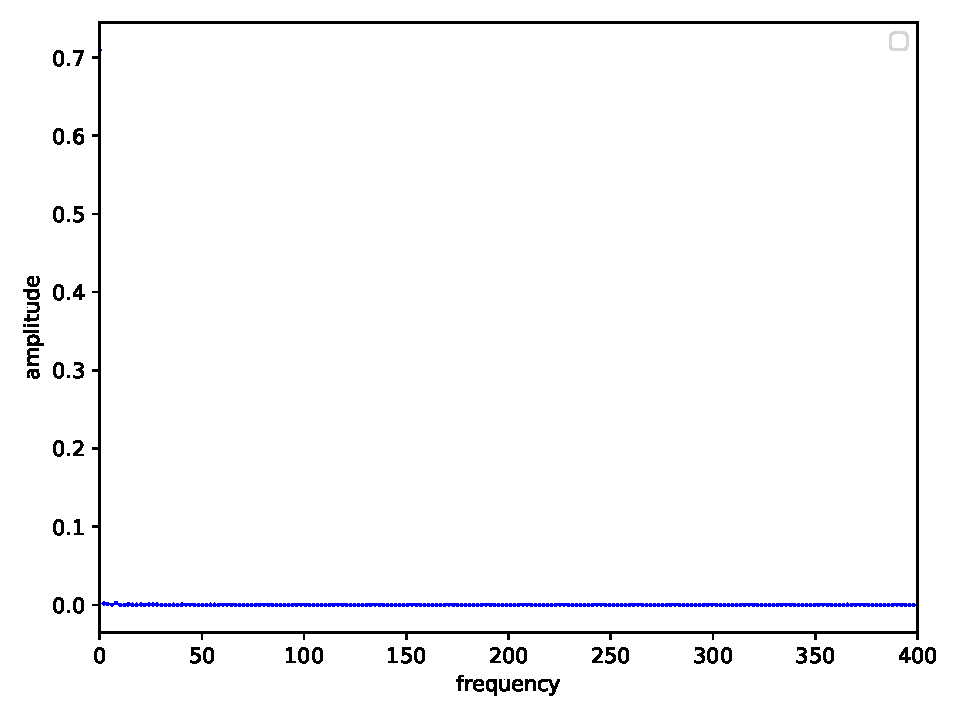
\includegraphics{plots/lomb_scarg.pdf}
    \caption{Lomb-Scargle periodogram.}
    \label{fig:lombscarg}
\end{figure}

\subsection*{(c)}

Taking a closer look at \autoref{fig:lombscarg} we can clearly see how the frequencies at lower values grow larger in amplitude, hinting at strong
daily, leading back to the usually large differences in temperatures during the day and night, and monthly fluctuations, which  can be explained by looking at different days in the same season 
- those tend to have around the same temperatures. \\

Furthermore, we see peaks where one would expect a year to have passed. This makes sense as well, as the temperatures tend to follow
the same trend for repeating seasons. \\

\subsection*{(d)}

First, we grid the data as can be seen in \autoref{list:gridding}.

\begin{lstlisting}[language = Python, caption={Data gridding.}, label = {list:gridding}]
    def resampled_fuction(x, x_orig, y_orig):
    interp = interp1d(x_orig, y_orig)
    return interp(x)

    gridded_x = np.linspace(2000,2008.9999620210326, len(M_scarg_2))
    tofou = resampled_fuction(gridded_x, M_scarg_2,T_scarg_2)
\end{lstlisting}

Then, we Fourier transform the new gridded data as seen in \autoref{list:furie}, which results in \autoref{fig:fourier}.

\begin{lstlisting}[language = Python, caption={Implementation of the Fourier transformation.}, label = {list:furie}]
    A_signal_gridded = rfft(tofou)
    frequencies = rfftfreq(np.size(gridded_x),1/365)
\end{lstlisting}

\begin{figure}[H]
    \centering
    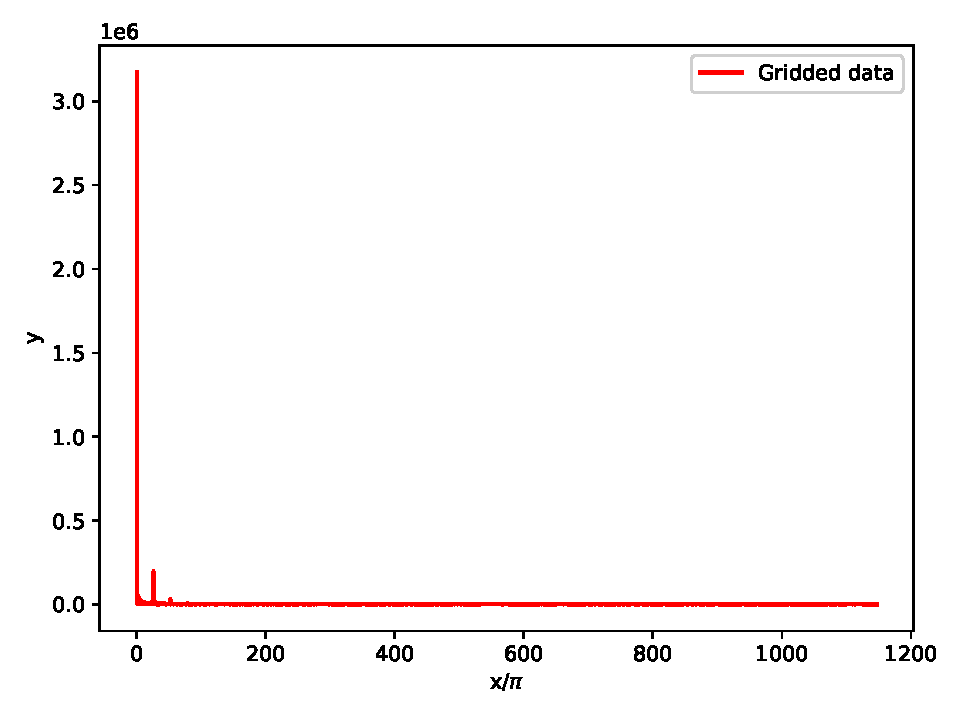
\includegraphics{plots/furie.pdf}
    \caption{Fourier transformation for the gridded data.}
    \label{fig:fourier}
\end{figure}

\subsection*{(e)}

Lastly, we isolate the two highest amplitude frequencies, which are conveniently the first two entries, so that we get \autoref{fig:e}.

\begin{figure}
    \centering
    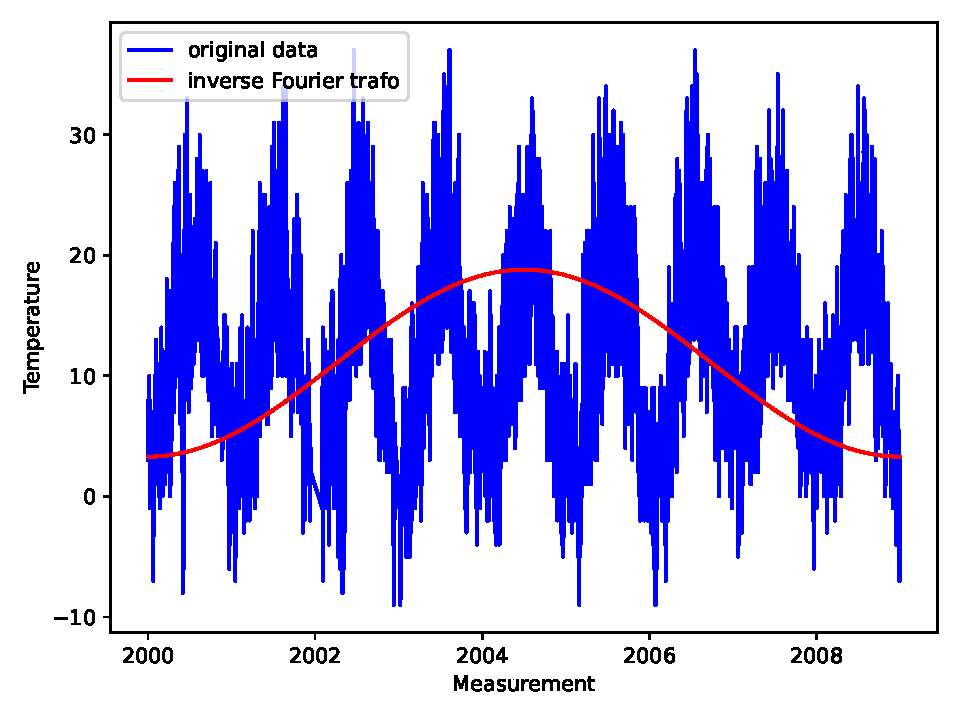
\includegraphics{plots/e.pdf}
    \caption{The plot for task (e).}
    \label{fig:e}
\end{figure}

That's probably not what it is supposed to look like.